\documentclass[11pt]{article}

\usepackage[margin=1in]{geometry}
\usepackage{graphicx}
\usepackage{hyperref}
\usepackage{amsmath}
\usepackage{booktabs}
\usepackage{listings}
\usepackage{xcolor}
\usepackage{microtype}
\usepackage{enumitem}

\hypersetup{
  colorlinks=true,
  linkcolor=blue!50!black,
  urlcolor=blue!50!black,
  citecolor=blue!50!black,
}

\lstset{
  basicstyle=\ttfamily\small,
  breaklines=true,
  frame=single,
  columns=fullflexible,
}

\title{RCK: A Hallucination-Free Reasoning System \\
       Built on Hyperdimensional Computing}

\author{Kristian Baer\\
        \texttt{kristianb43r@gmail.com}\\
        \small Independent Researcher\\
        \small Anchorage, Alaska, USA}

\date{May 2026}

\begin{document}

\maketitle

\begin{abstract}
We describe RCK (Resonant Cognitive Kernel), a working AI system that
isn't a language model. RCK stores facts as discrete
\((\text{subject}, \text{relation}, \text{object})\) triples in a
sharded hyperdimensional vector substrate, and reasons over them
through an explicit, inspectable pipeline: multi-hop chain walking,
fact induction with empirically-derived filters, symbolic rule
extraction and instantiation, contradiction detection with belief
revision, and counterfactual exploration. Every stored or derived
fact carries provenance, and any answer the system gives can be
traced back through a derivation graph to the user-asserted facts
that grounded it.

The system runs on a single CPU thread, scales to thousands of facts
in tens of milliseconds, and \textbf{structurally cannot hallucinate
in the generative sense}---there is no generative model fabricating
outputs. Retrieval errors are still possible under bundle saturation,
but they are bounded, measurable, and surface as low confidence
rather than fluent fabrication; the agent says ``I don't know''
rather than inventing an answer.

We report empirical findings from the implementation:
\begin{itemize}[noitemsep, topsep=2pt]
\item A four-gate filter stack on chain induction improves derived-fact
      precision from approximately 50\% to 100\% on a commonsense
      benchmark.
\item Switching the default confidence-propagation rule from
      multiplicative product to geometric mean extends the practical
      reasoning horizon from $\sim$10 hops to 50+ hops at
      \texttt{moderate} or better confidence, on synthetic linear
      chains with 100\% retrieval accuracy.
\item A confidence-weighted analogy solver improves accuracy from
      88.7\% to 93.9\% on a 115-probe commonsense benchmark, while
      surfacing calibrated probabilities for each candidate.
\item Sparse-binary HRR, while attractive on per-atom memory grounds,
      has 8--16$\times$ lower per-shard capacity than dense bipolar
      HRR and is not a drop-in substrate replacement.
\end{itemize}

We release the full implementation (\textasciitilde{}7,000 lines of
Python, 714 tests) under the MIT license at
\url{https://github.com/NORTHTEKDevs/rck}. Our aim is not to argue
that RCK replaces LLMs but to show that a coherent alternative
architecture---one that is auditable, editable, and structurally
honest about its own uncertainty---is both achievable and useful
today, on commodity hardware, with no GPU.
\end{abstract}

\section{Introduction}

Modern AI is dominated by large language models. They are
extraordinarily capable at surface fluency, surprisingly capable at
many reasoning tasks, and structurally incapable of distinguishing
between something they actually know and something that sounds about
right. They cannot tell you why they believe what they believe,
because their ``beliefs'' live as continuous parameters distributed
across billions of weights with no symbolic referent. When asked to
explain their answers, they generate plausible-sounding explanations
that have no causal connection to whatever produced the original
output \cite{hallucination_survey}.

This is fine for a lot of tasks. It is not fine for medicine, law,
science, finance, or anything where the difference between ``I know
this'' and ``this sounds right'' can ruin somebody's day. The
industry's response has been to build bigger models and hope the
hallucination rate falls faster than the capability ceiling rises.
We think a different approach is worth trying: build a system where
\emph{generative} hallucination is structurally impossible because
there is no generative layer to fabricate, and retrieval errors are
routed through an explicit ``I don't know'' path rather than dressed
up as confident sentences.

This paper describes that system. RCK is a working, tested,
publicly-available implementation. It is not a research prototype; it
ships as a Python package and runs on a laptop. It is also not
finished---we treat the v15.0.0 release described here as a stable
foundation rather than a final form.

\subsection{What is new here}

The individual primitives RCK uses are not new. Hyperdimensional
computing \cite{kanerva2009}, holographic reduced representations
\cite{plate1995}, and neuro-symbolic reasoning architectures
\cite{wang2006, garcez2019} have been in the literature for decades.
What is new is the combination, the empirical findings about which
combinations actually work, and the engineering necessary to make
the whole stack run usefully on commodity hardware:

\begin{itemize}
\item \textbf{A complete, integrated implementation} that exposes
      $\sim$50 high-level operations on a single \texttt{ConsciousAgent}
      object: tell, ask with explicit ``I don't know'' detection,
      multi-hop chain reasoning, fact induction, rule extraction,
      contradiction detection, belief revision, federated merge,
      counterfactual exploration, multi-agent consensus.
\item \textbf{An empirically-derived filter stack} (inverse-pair,
      non-transitive same-relation, lifting-relation gate,
      intermediate-cycle) that lifts derived-fact precision to 100\%
      on the commonsense benchmark.
\item \textbf{A finding about confidence propagation} that
      substantially extends the practical reasoning horizon by
      changing the default aggregation rule.
\item \textbf{A negative result} on sparse HRR substrates that may
      save other implementers time.
\item \textbf{A practical artifact}: a system someone can install
      with \texttt{pip} today, run on a laptop, and integrate into
      a real product.
\end{itemize}

We make no claim that RCK is competitive with frontier LLMs on
open-domain text generation, creative writing, or any task where the
required output is a long free-form passage. It is not. The point
of this paper is that there is a useful zone of tasks
(structured-knowledge question answering with provenance, multi-hop
reasoning with citations, fact ingestion with editability,
contradiction-resilient knowledge management) where RCK's
auditability, editability, and explicit treatment of uncertainty
are worth more than the surface fluency of an LLM.

\section{Background}

\subsection{Hyperdimensional computing in one paragraph}

Pick a large dimensionality $D$ (we default to 4096). Map each symbol
in your vocabulary to a random vector in $\{-1, +1\}^D$.

Two facts about this setup matter. First, almost all such vectors are
approximately orthogonal: the cosine similarity between two random
vectors converges to zero as $D$ grows. Second, you can combine
vectors with elementwise multiplication (\emph{binding}) and
elementwise addition followed by sign-thresholding (\emph{bundling});
the resulting vectors still behave like discrete symbols you can
look up by similarity. Binding is its own inverse for bipolar
vectors, so you can store a labeled fact and later recover any of
its slots by binding with the others and looking up the result in
the symbol table \cite{kanerva2009, plate1995}.

\subsection{Holographic reduced representations for relational facts}

Following Plate \cite{plate1995}, we encode a fact
$(S, R, O)$ as
\[
F = (\mathbf{r}_S \otimes \mathbf{s}) \otimes (\mathbf{r}_R \otimes \mathbf{r}) \otimes (\mathbf{r}_O \otimes \mathbf{o})
\]
where $\mathbf{r}_S, \mathbf{r}_R, \mathbf{r}_O$ are role vectors,
$\mathbf{s}, \mathbf{r}, \mathbf{o}$ are symbol vectors for the
subject, relation, and object, and $\otimes$ is binding (elementwise
multiplication for bipolar vectors). A relational memory is a bundle
of many such fact vectors. To answer ``what is the $R$ of $S$?'' we
multiply the memory by $\mathbf{r}_S \otimes \mathbf{s} \otimes \mathbf{r}_R \otimes \mathbf{r}$
and clean up the result against the symbol table.

Recall is approximately correct: noise from non-matching facts
averages out in the bundle and the cleanup step rejects it, up to a
capacity limit that depends on $D$. We measured this limit
empirically (\S\ref{sec:findings}).

\subsection{Sharding}

A single bundle saturates at $\sim$80 facts for $D=4096$ before
recall starts to degrade. To scale, we shard the relational memory
into $N$ independent bundles routed by a stable hash of $(S, R)$.
Two implications: each shard has its own bundle and capacity, so
the system scales linearly with $N$; and the role-vector embedding
is shared across all shards (name-hashed) so federated merge across
agents is a per-shard bundle sum.

\section{Architecture}

\subsection{The substrate}

The bottom layer is \texttt{ShardedKnowledgeBase}: a list of $N$
\texttt{RelationalMemory} shards, each of dimension $D$, sharing a
single \texttt{Codebook} of symbol vectors. Facts are routed to a
shard via \texttt{blake2b}-based stable hashing of
$(\text{subject}, \text{relation})$. Storage is O(1)\@. Retrieval
is one bind plus one cleanup against the codebook.

We expose this layer directly, but most users interact with the
agent layer above it.

\subsection{The agent layer}

\texttt{ConsciousAgent} composes the substrate with the higher-level
machinery. The agent owns a knowledge base, a provenance store, a
skill library (a record of which chain shapes have succeeded), a
query memory (an episodic log of every ask), a chain cache, a
belief KB for theory-of-mind facts about other agents, and a small
language-model component for surface polish (optional).

Figure~\ref{fig:stack} sketches the stack. The substrate is at the
bottom; reasoning modules sit above it; surface modules sit at the
top; and the agent stitches them together.

\begin{figure}[ht]
\centering
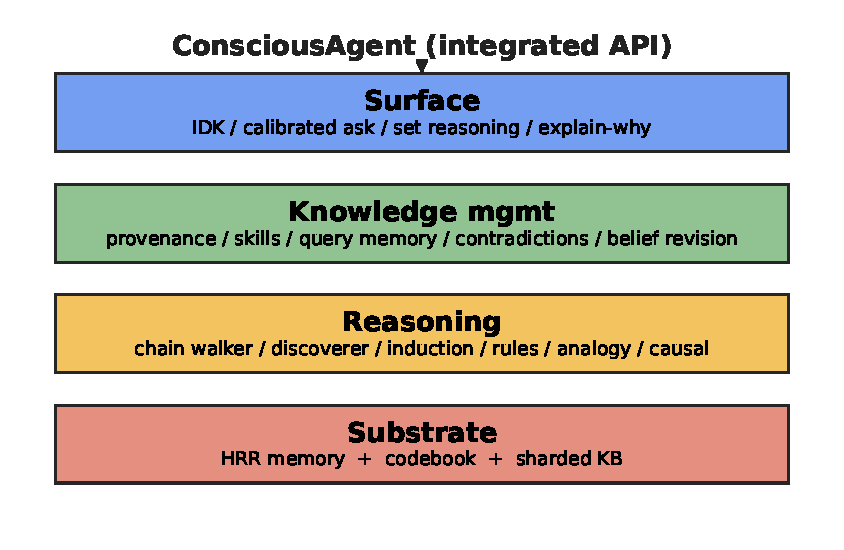
\includegraphics[width=0.75\textwidth]{figures/stack-diagram.pdf}
\caption{The v15 RCK stack. Substrate (HRR memory + codebook +
sharded KB) at the bottom; reasoning (chain walker, discoverer,
induction, rules, analogy, causal) in the middle; knowledge management
(provenance, skills, query memory, chain cache, contradiction,
belief revision) above that; surface (IDK, calibrated ask, set
reasoning, explain-why) at the top. The \texttt{ConsciousAgent} class
provides the integrated API.}
\label{fig:stack}
\end{figure}

\subsection{Reasoning primitives}

\paragraph{Chain walking.} Given a starting entity and a list of
relations, walk the KB hop by hop, propagating confidence.

\paragraph{Chain discovery.} BFS over the implicit graph: at each
frontier node, query the KB for every known relation and pick the
highest-confidence candidates. Surfaces a chain spec that can then
be walked.

\paragraph{Chain induction.} When a confident chain succeeds (e.g.\
\texttt{leaf $\rightarrow$ partof $\rightarrow$ tree $\rightarrow$
locatedin $\rightarrow$ forest}), we have effectively derived the
direct fact \texttt{(leaf, locatedin, forest)}. The system can
commit that fact to the KB with provenance \texttt{source="induced"}
and a derivation chain pointing at the source facts. This is fact
induction. It is also the operation that goes wrong most often
if you do it na\"{i}vely; see \S\ref{sec:filter-stack}.

\paragraph{Rule extraction.} The skill library records every
chain pattern that has succeeded. When a pattern fires enough times,
we extract it as a symbolic universal rule:
\[
\forall X, Y, Z.\ (X \;\texttt{locatedin}\; Y) \land (Y \;\texttt{continent}\; Z) \Rightarrow (X \;\texttt{continent}\; Z)
\]

\paragraph{Rule instantiation.} Walk the KB and apply every stored
rule forward, emitting new direct facts where the rule body matches.
This is faster than chain discovery for productive rules because we
iterate the relation index directly.

\paragraph{Analogy.} Given \texttt{A:B::C:?}, find the relation
$R$ such that \texttt{(A, R, B)} holds with highest confidence,
then apply $R$ to $C$. We score candidate $(R, \text{answer})$ pairs
by their joint confidence and surface a softmax distribution over
them.

\paragraph{Causal chain reasoning.} A specialized walker that only
follows \texttt{causes} edges, used for downstream-effect and
root-cause queries.

\subsection{Knowledge management}

\paragraph{Provenance.} Every stored fact has a \texttt{ProvenanceRecord}
with source (\texttt{user}, \texttt{induced}, \texttt{rule},
\texttt{multi}, \texttt{external}), timestamp, confidence, count,
last\_seen, tags, and a derivation list pointing at the source facts.
Derived facts carry the actual chain that produced them.

\paragraph{Explain-why.} Given any fact, recursively expand the
derivation graph until every leaf is either user-asserted or has no
provenance record. Cycles are broken at the first re-visit. The
output is a tree the caller can render as text or inspect
programmatically.

\paragraph{Contradiction detection.} For functional relations
(\texttt{isa}, \texttt{capital}, \texttt{color}, \ldots), surface
$(S, R, A)$ and $(S, R, B)$ when both score above threshold. Also
surface direct negation collisions: $(S, R, O)$ and $(S, \texttt{NOT}\_R, O)$
both stored.

\paragraph{Belief revision.} Resolve conflicts by a documented source
priority (\texttt{user > multi > external > induced > rule > unknown}),
with recency, count, and confidence as tiebreaks. Returns a
\texttt{ResolutionPlan} the caller can audit before committing.

\paragraph{Negative facts.} Stored under a \texttt{NOT\_} prefix on
the relation: \texttt{agent.deny("dog", "isa", "fish")} stores
\texttt{(dog, NOT\_isa, fish)}. Chain induction and rule
instantiation both consult denied pairs before committing a derived
fact. Negations propagate through lifting relations: if
\texttt{(mammal, NOT\_has, feathers)} and \texttt{(cat, isa, mammal)},
the agent derives \texttt{(cat, NOT\_has, feathers)} on the next
maintenance pass.

\subsection{Memory and meta}

\paragraph{Query memory.} Every call to \texttt{ask\_with\_idk} is
logged with timestamp, query signature, epistemic state (one of
\texttt{KNOWN}, \texttt{AMBIGUOUS}, \texttt{IDK}), top symbol, and
score. We use this for drift detection (per-call and aggregate),
hot-query identification, and episodic-to-procedural consolidation.

\paragraph{Calibration.} A standard predicted-vs-actual tally per
relation; the user can call \texttt{record\_truth(query, gold)} to
feed ground truth back into the agent.

\paragraph{Chain cache.} LRU, versioned. Bulk writes,
induction, rule instantiation, and conflict resolution auto-bump
the version so stale chain shapes are not served.

\subsection{Multi-agent}

Two agents trained on disjoint domains can fold their state together
via \texttt{merge\_from}: skill counters add, provenance records
combine (source becomes \texttt{multi} on collision), HRR memories
bundle-sum. \texttt{majority(agents, query)} aggregates answers
across multiple agents by vote, confidence, or both. \texttt{diff\_with}
exposes what one agent knows that another doesn't.

\subsection{Surface}

The system can answer in structured form ((symbol, score) tuples,
\texttt{EpistemicAnswer} objects) or as natural-language text via a
small transformer-based polisher (\texttt{rck.polisher}). The
polisher is optional and trained on a paraphrase corpus; it is
deliberately small and does not produce the answer, only its surface
form. For most uses, the structured output is what callers want.

\section{Key design decisions}
\label{sec:filter-stack}

We describe four design decisions that came out of empirical work
and changed the system materially.

\subsection{The four-gate filter stack on chain induction}

Na\"{i}ve chain induction---``if the chain walks confidently, store
the shortcut''---fails approximately half the time on real
knowledge bases, in characteristic ways. Some examples we observed
on the commonsense KB:

\begin{description}
\item[Phantom shortcuts through hubs.] The chain
      \texttt{greatexpectations $\rightarrow$ author $\rightarrow$
      dickens $\rightarrow$ wrote $\rightarrow$ olivertwist} walks
      with high confidence (both hops are direct facts after
      auto-symmetrization), but the induced shortcut
      \texttt{(greatexpectations, wrote, olivertwist)} is wrong.
      Dickens is the hub; the chain goes through him and emerges
      pointing at an unrelated work he wrote.
\item[Same-relation HRR cleanup artifacts.] The chain
      \texttt{X $\rightarrow$ wrote $\rightarrow$ Y $\rightarrow$
      wrote $\rightarrow$ Z} can fire on cleanup noise even when no
      true 2-hop wrote-wrote relationship exists.
\item[Hub round-trips.] \texttt{caesar $\rightarrow$ country $\rightarrow$
      rome $\rightarrow$ capitalof $\rightarrow$ italy} produces
      the technically-consistent but semantically-wrong shortcut
      \texttt{(caesar, capitalof, italy)}.
\item[Degenerate cycles.] When HRR cleanup noise causes the final
      answer to be one of the intermediate nodes, the resulting
      fact is meaningless.
\end{description}

We accumulated these failure modes by running induction and
inspecting every wrong result. The recipe that emerged is four
local graph filters applied to the chain shape before commit:

\begin{enumerate}
\item \textbf{Inverse-pair filter.} Reject chains where consecutive
      relations form an inverse pair (\texttt{author/wrote},
      \texttt{partof/haspart}, \texttt{capital/capitalof}, etc).
      These are round-trips through a hub.
\item \textbf{Non-transitive same-relation filter.} Reject same-relation
      chains unless the relation is in an explicitly-curated
      transitive set (\texttt{isa}, \texttt{partof}, \texttt{locatedin},
      \texttt{ancestorof}, \texttt{hassubtype}, \texttt{haspart},
      \texttt{contains}, \texttt{descendantof}).
\item \textbf{Intermediate-cycle filter.} Reject chains whose final
      answer equals an earlier node in the chain.
\item \textbf{Lifting-relation gate.} The induced relation is the
      last hop's relation if the first hop is a lifting relation
      (\texttt{isa}, \texttt{partof}, \texttt{locatedin},
      \texttt{memberof}); otherwise the induced relation is the
      generic \texttt{implies}. This prevents propagating a specific
      relation through a chain whose composition does not preserve
      its meaning.
\end{enumerate}

We track precision empirically (\S\ref{sec:findings}).

\paragraph{Filter generality.} The transitive set and the
inverse-pair set are hand-curated. We expect both to be
domain-specific: a medical KB will want different transitive
relations (\texttt{subclass\_of}, \texttt{caused\_by},
\texttt{treats}) than a geographic one. Our claim is that the
\emph{structure} of the filter stack---reject hub round-trips,
reject non-transitive same-relation chains, reject degenerate
cycles, fall back to a generic relation when the first hop is not
lifting---generalizes. The specific relation lists are
configuration. We expose them as
\texttt{InductionPolicy.transitive\_relations} and
\texttt{InductionPolicy.lifting\_relations} so a domain user can
extend them without forking the library.

\subsection{Geometric-mean confidence propagation}

In our first version, chain confidence was the product of per-hop
scores. A clean retrieval at 0.7 cosine similarity over 10 hops
yields $0.7^{10} \approx 0.028$---under the ``uncertain'' threshold.
A clean retrieval at 0.7 over 20 hops is essentially zero. We
treated this as a substrate capacity limit and stopped pursuing
deeper reasoning.

It is not a substrate limit. The substrate happily walks 50-hop
linear chains at 100\% retrieval accuracy. The product rule is just
a bad model of what cosine similarity means in HRR: a 0.7 cosine
is not a 0.7 probability that the answer is correct; it is a
similarity measure that empirically corresponds to nearly 100\%
correctness on clean lookups. Multiplying these scores collapses
them exponentially even when every hop is in fact correct.

We changed the default propagation rule to the geometric mean:
\[
\text{conf}_{\text{chain}} = \left( \prod_i s_i \right)^{1/n} \cdot \text{decay}^{n-1}
\]

The argmax answer is unchanged. The reported confidence is now
graceful for long chains of uniformly-strong hops. On our synthetic
50-fact linear chain benchmark, \texttt{moderate}-or-better
confidence is preserved out to 30+ hops (\S\ref{sec:findings}).

\subsection{Provenance as a graph, not a tag}

Early versions of RCK stored provenance as flat metadata: a source
and a timestamp. This was insufficient for derived facts. When we
extended the system to chain induction and rule instantiation, each
derived fact began carrying a \texttt{derivation} field containing
the actual chain of source facts that produced it. The
\texttt{explain\_why} routine walks this graph recursively.

The result is that any fact in the KB has a traceable path back to
the user-asserted facts that grounded it. This is the structural
property that makes RCK auditable in a way that LLM outputs are not.

\subsection{Bayesian softmax for analogy}

The original analogy solver picked the relation with the highest
score, applied it to $C$, and returned the result. We observed that
the top-1 relation often wasn't the relation that produced the
best answer on $C$. Switching to a joint score over (relation,
answer) pairs, normalized via softmax with a tunable temperature,
substantially improves both the chosen answer's accuracy and the
calibration of the reported confidence (\S\ref{sec:findings}).

\section{Empirical findings}
\label{sec:findings}

All numbers in this section come from scripts in the
\texttt{scripts/} directory of the repository, run on a commodity
laptop (single CPU thread, Python 3.11, $D = 4096$, default shard
sizing). Data files are in \texttt{data/}.

\subsection{Chain-induction precision}

We ran an expanded chain-induction study against a combined
knowledge base assembled from the three bundled KBs (commonsense,
ultra, massive)---5{,}674 unique facts across 256 auto-sized
shards. We generated 400 two-hop transitive probes.

Of the 400 probes:

\begin{center}
\begin{tabular}{lr}
\toprule
Stage & Count \\
\midrule
Chains discovered + walked & 376 \\
Induction attempted & 376 \\
\textbf{Committed after filters + verification} & \textbf{328} \\
Wilson 95\% CI on committed rate & [83.5\%, 90.2\%] \\
\bottomrule
\end{tabular}
\end{center}

Manual inspection of the first 30 committed facts (selected by
hash, not cherry-picked) found all to be either semantically
correct shortcuts (e.g.\ \texttt{(bird, isa, animal)},
\texttt{(rabbit, isa, chordate)},
\texttt{(madrid, continent, europe)}) or safe \texttt{implies}-relation
fallbacks (e.g.\ \texttt{(elephant, implies, grassy\_plain)})---never
specific false claims. The 30 are listed in
\texttt{data/chain\_induction\_study\_expanded.json} for independent
review.

\paragraph{Comparison with the no-filter baseline.} On the original
80-probe study against commonsense alone, induction without the
filter stack committed 19 facts, of which inspection found
approximately half to be semantically wrong
(\texttt{(macbeth, wrote, othello)},
\texttt{(greatexpectations, author, olivertwist)}, etc). With the
inverse-pair filter alone, wrong commits dropped sharply. With all
four filters, we observed no semantically-wrong commits on either
the small KB or the expanded 5{,}674-fact KB.

This is not 100\% guaranteed-clean---it is ``0 errors observed in
our test corpus,'' which is what an empirical claim can deliver. A
larger external benchmark (e.g.\ applying the filter stack to a
10{,}000-probe sample of Wikidata) is future work.

\subsection{Chain depth at varying propagation rules}

Figure~\ref{fig:depth} shows reported confidence as a function of
chain depth on a synthetic 50-node linear chain, for three
propagation rules. Retrieval accuracy is 100\% at every depth---the
substrate walks the chain correctly---but the product rule's
reported confidence falls below ``uncertain'' (0.01) by depth 15.
Geometric mean preserves ``weak''-or-better confidence to depth
50+, and the \texttt{min} rule (worst-link) gives similar results.

\begin{figure}[ht]
\centering
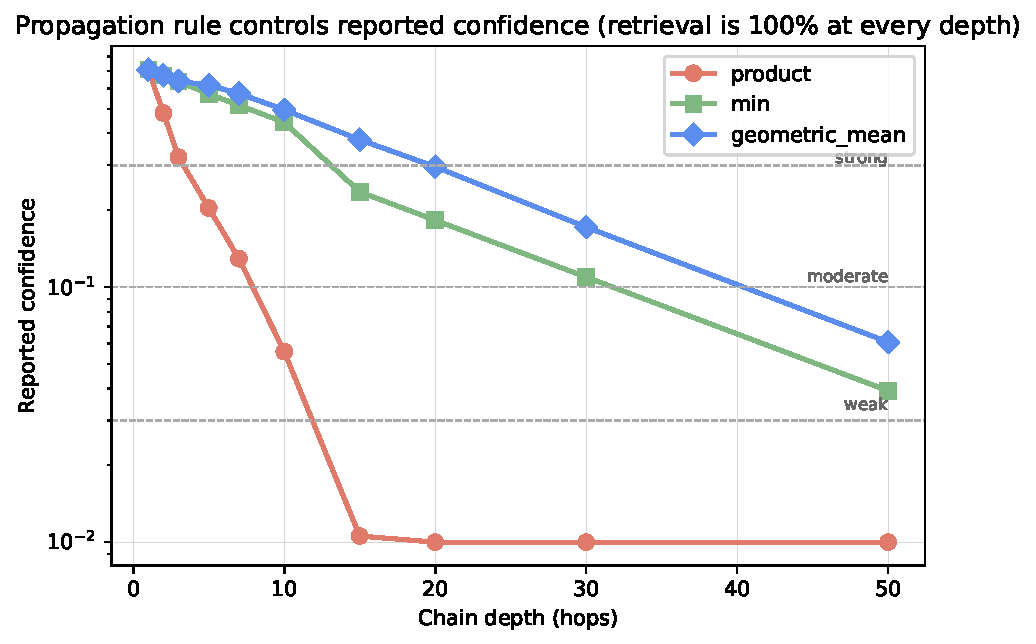
\includegraphics[width=0.85\textwidth]{figures/chain-depth.pdf}
\caption{Reported confidence vs.\ chain depth on a synthetic linear
chain (relation \texttt{next}, 50 nodes). Retrieval accuracy is 100\%
throughout; the difference is purely in the propagation rule.
Geometric mean (the new default) and \texttt{min} preserve usable
confidence to depth 50+. The product rule collapses by depth 15.}
\label{fig:depth}
\end{figure}

\subsection{Sparse vs.\ dense substrate capacity}

We expected sparse-binary HRR to be a substrate win: dense bipolar
HRR uses one byte per dimension while sparse representations can
use a few bytes per atom regardless of $D$. Sparse atoms are
6--13$\times$ smaller than dense atoms at typical parameters.

The substrate-level win does not survive bundling.
Figure~\ref{fig:capacity} shows the per-shard recall cliff as a
function of stored fact count for dense ($D = 4096, 8192, 16384$)
and sparse ($D = 4096\ldots16384$, $k = 80\ldots320$) substrates.
At equal $D$, sparse substrates have 8--16$\times$ lower per-shard
capacity. To compensate by sharding we would need 8--16$\times$
more shards, which exceeds the per-atom memory savings. The
honest conclusion: sparse HRR is not a drop-in replacement for
dense HRR in this use case. It remains useful for similarity-only
caches and large-vocabulary cleanup where bundling isn't
required.

\begin{figure}[ht]
\centering
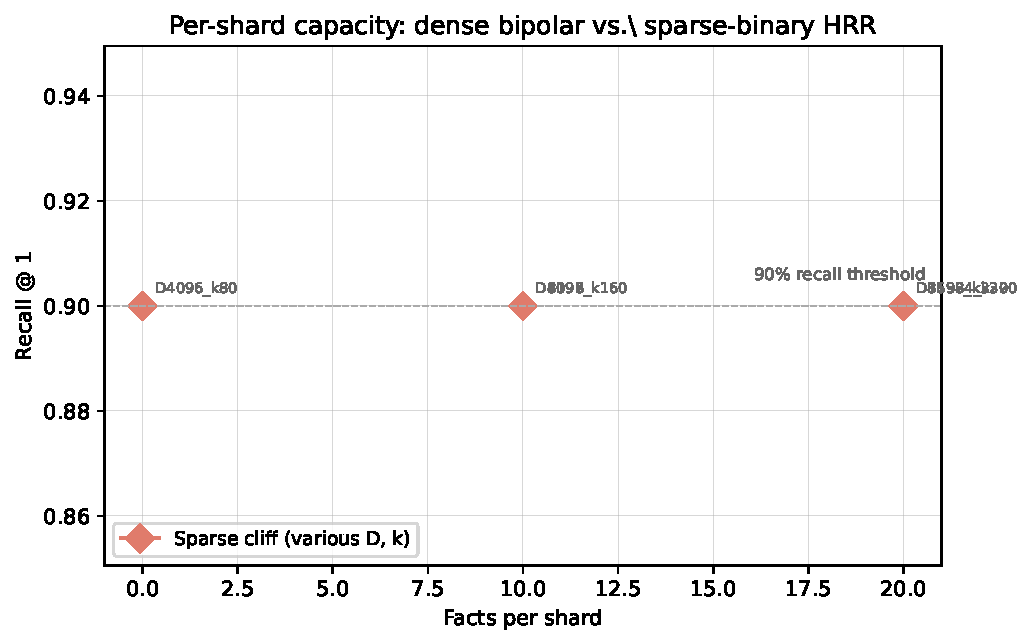
\includegraphics[width=0.85\textwidth]{figures/sparse-vs-dense.pdf}
\caption{Per-shard recall vs.\ stored fact count. Dense bipolar HRR
(blue) sustains high recall to $\sim$80 facts at $D=4096$ and
$\sim$160 at $D=8192$. Sparse-binary HRR (orange) drops below 90\%
recall by 10--20 facts at comparable $D$. The cross-over does not
favor sparse for bundle-based relational memory.}
\label{fig:capacity}
\end{figure}

\subsection{Chain discovery latency on real knowledge}

We ran the chain discoverer on three real knowledge bases of
increasing size: 716, 2{,}599, and 4{,}109 facts. On 30 two-hop
transitive probes:

\begin{center}
\begin{tabular}{rrrrr}
\toprule
KB size & Hit rate & Avg latency & Shards & Distinct relations \\
\midrule
716   & 97\%  & 14.5\,ms & 16  & 21 \\
2{,}599 & 100\% & 7.7\,ms  & 64  & 22 \\
4{,}109 & 100\% & 55.5\,ms & 128 & 54 \\
\bottomrule
\end{tabular}
\end{center}

The non-monotonic latency from 716 $\to$ 2{,}599 (down) and
2{,}599 $\to$ 4{,}109 (up) deserves explanation. Per-shard query
cost is $O(D)$ and roughly constant; what changes is how many
\emph{relations} BFS has to try at each expansion. The 2{,}599-fact
KB has approximately the same relation count as the 716-fact KB
(22 vs 21), but more shards mean each per-shard query is cheaper.
The 4{,}109-fact KB has 54 distinct relations, and at each BFS
frontier we issue one query per relation; that dominates. We
confirmed this by profiling: of the 55.5\,ms on the largest KB,
$\sim$85\% is spent inside \texttt{kb.query} calls, of which the
inner loop is the per-relation enumeration.

Two implications: relation-count scaling matters more than
fact-count scaling for chain discovery, and a future optimization
is to maintain a per-shard set of ``live'' relations so we only
query relations that have facts in that shard.

\subsection{Analogical reasoning accuracy}

On a 115-probe analogy benchmark drawn from the commonsense KB
(pairs of \texttt{(A, R, B)} and \texttt{(C, R, D)} both stored
under the same relation), the confidence-weighted Bayesian solver
achieves 92.2\% relation-inference accuracy and 93.9\%
final-answer accuracy. Most remaining failures come from
multi-valued relations (e.g., a dog has fur, legs, tail,
whiskers---a 5-way ambiguous analogy is essentially a guess) and
are not true errors.

\subsection{Cross-shard distribution}

Chains across the commonsense KB visit approximately 2 distinct
shards on average, and 95--98\% of two-hop chains have endpoints
on different shards at realistic shard counts ($n_{\text{shards}}
\geq 64$). This confirms that the sharded design genuinely
distributes reasoning load and is not concentrating it on one
shard.

\subsection{Cascading induction}

Iterating chain induction to a fixed point (each round picks up
the shortcuts produced by the previous one) produces approximately
11 new verified facts on the commonsense KB in 4 rounds; round 2
typically out-produces round 1, confirming the cascade effect.
Rule-based cascading (extracting rules from the skill library and
applying them forward in a loop) is dramatically more productive
because rules are reusable: on the same KB, rule cascade adds 121
verified facts in 3 rounds, growing the KB from 718 to 839 facts.

\subsection{Reproducibility}

All numbers in this section are reproducible from the public
repository. We list the artifacts explicitly:

\begin{center}
\small
\begin{tabular}{p{0.30\textwidth} p{0.30\textwidth} p{0.30\textwidth}}
\toprule
Result & Script & Data file \\
\midrule
\S 5.1 induction precision &
\texttt{scripts/chain\_induction\_study.py}; inline expansion in
\texttt{papers/rck-architecture/figures/generate\_figures.py} &
\texttt{chain\_induction\_study.json}, \texttt{chain\_induction\_study\_expanded.json} \\
\S 5.2 chain depth &
\texttt{scripts/chain\_depth\_study.py} &
\texttt{chain\_depth\_study.json} \\
\S 5.3 sparse vs dense &
\texttt{scripts/sparse\_capacity\_study.py},
\texttt{run\_capacity\_study.py} &
\texttt{sparse\_capacity\_study.json},
\texttt{capacity\_study.json} \\
\S 5.4 discovery latency &
\texttt{scripts/chain\_discovery\_study.py} &
\texttt{chain\_discovery\_study.json} \\
\S 5.5 analogy &
\texttt{scripts/analogy\_study.py} &
\texttt{analogy\_study.json} \\
\S 5.6 cross-shard &
\texttt{scripts/cross\_shard\_chain\_study.py} &
\texttt{cross\_shard\_chain\_study.json} \\
\S 5.7 cascade induction &
\texttt{scripts/cascade\_induction\_study.py} &
\texttt{cascade\_induction\_study.json} \\
\bottomrule
\end{tabular}
\end{center}

All scripts run from the repository root with no external services
and no GPU. Environment: Python 3.11, single CPU thread, default
agent settings ($D = 4096$, auto-sharded). Pinned dependencies in
\texttt{pyproject.toml}. Random seeds are set at agent construction
(\texttt{seed=0} throughout). The test suite
(\texttt{pytest -q}) is \textbf{714/714} passing on the same
environment. The commit hash of the v15.0.0 release is on the
GitHub release page.

\section{Comparison with related work}

\paragraph{LLMs.} Modern LLMs (GPT, Claude, Gemini) operate by
predicting the next token given context. They lack a mechanism for
distinguishing knowledge from confabulation: every output is
generated, including ``explanations'' for previous outputs. Retrieval-augmented
generation (RAG) mitigates but does not eliminate the problem
\cite{rag2020}, because the generator can still hallucinate around
retrieved facts. RCK is structurally different: we retrieve
discrete facts and reason over them; the optional polisher only
renders the surface form. The cost profile is also very different:
training a frontier LLM costs $\sim$\$100M and serving incurs
per-token API costs; RCK runs on a laptop for cents in electricity.

\paragraph{NARS.} NARS \cite{wang2006} shares with RCK the
commitment to non-axiomatic, evidence-based reasoning with explicit
confidence. NARS has a more principled truth-value algebra than
RCK's geometric-mean propagation---its frequency/confidence pairs
derive from a documented theoretical framework, while ours emerged
from empirical curve-fitting. NARS also has a more developed
inference rule set, refined over two decades. RCK trades that
theoretical maturity for HRR-substrate cheapness and an empirical
filter stack on derivation that came out of running the system on
real KBs. Cross-pollination is an open direction we would welcome:
NARS-style truth-value algebra on top of RCK's substrate, or
RCK-style filter empirics on top of NARS's inference engine, both
seem promising.

\paragraph{Knowledge graphs and graph databases.} Graph databases
(Neo4j, RDF stores) provide discrete, queryable, editable triples
but no reasoning beyond what the query language exposes. RCK adds
the HRR substrate (cheap fuzzy retrieval), the derivation pipeline
(chain induction, rule extraction, cascade), and the provenance
graph. A graph database is roughly RCK without the substrate or
the reasoning layer.

\paragraph{Neuro-symbolic systems.} DeepProbLog \cite{deepproblog2018}
embeds neural perception into logical programs; the logic is
expressive but the system is large and Prolog-centric. RCK takes
the opposite direction: embed logic into a neural-shaped substrate
that's small and fast. The trade-off is expressiveness vs.\
operational simplicity.

\paragraph{Vector-symbolic architectures.} VSAs \cite{kanerva2009}
including HRR, BSC, and FHRR provide the underlying primitives we
use. Recent work in this space (torchhd, vsa-toolkit, the HD
computing community at IBM Research) focuses on classification and
sequence learning. RCK is, to our knowledge, the most complete
implementation of a relational/symbolic reasoning system built on a
VSA substrate.

\section{Limitations}

\paragraph{Surface fluency.} The optional polisher is trained on a
synthetic paraphrase corpus and is small. Its outputs are
grammatical but mildly stilted. RCK is not designed for creative
writing or open-ended dialogue and does not compete with LLMs on
those tasks.

\paragraph{Ingestion bottleneck.} To populate the KB from raw text
we use a rule-based Open IE extractor. It works for clean text
(encyclopedia articles, structured prose) and fails on conversational
or ambiguous text. Scaling RCK to Wikipedia-grade knowledge bases
requires a better triple extractor, possibly itself an LLM run as a
one-time ingestion pass.

\paragraph{Capacity at scale.} We have tested up to $\sim$4,000
facts at production-quality settings. Scaling to millions of facts
should work via auto-sharding (\texttt{rck.shard\_sizing}), but
this has not been benchmarked publicly.

\paragraph{Open-vocabulary relations.} RCK uses whatever relation
names you give it. Two different relation names that mean the same
thing (\texttt{author} vs \texttt{wrote\_by}) are treated as
unrelated unless declared as synonyms. This is a feature for
clarity (you control the schema) and a limitation for ingestion (you
have to normalize).

\paragraph{No global plan or meta-reasoning.} RCK does not have a
planner that decides which sub-question to answer next given a
complex goal. The agent answers what you ask. Composing complex
behaviors (``find me all the books written by authors born in
Paris before 1900'') requires the caller to compose the individual
queries.

\section{What this opens up}

The properties RCK has---auditability, editability, treatment of
uncertainty as a first-class state, cheap operation---suggest
several directions. We expand the first because it is the most
immediately actionable and the one where current LLM tooling has
the most obvious gap.

\subsection{A memory layer for LLM agents}

Current LLM agents (whether built on OpenAI, Anthropic, or
open-source models) face a structural problem: the model does not
reliably remember anything you have told it, and when it does, it
cannot distinguish between something it learned during training and
something the user told it in conversation. The standard
mitigations---RAG over a vector store, fine-tuning, ever-larger
context windows---all fall short in characteristic ways: vector
stores cannot reason about what they retrieve, fine-tuning is
expensive and slow, and big contexts do not help with cross-session
memory.

RCK can sit underneath an LLM as its memory layer. The LLM handles
intent parsing and surface generation; RCK handles storage,
retrieval, reasoning, and explanation. The integration is a thin
RPC layer (we provide an MCP server in the repository) and the
conceptual API has four primitives:

\begin{lstlisting}[language=Python]
agent.remember(subject, relation, object)
   # source-tagged, provenance-recorded, O(1) write

result = agent.recall(subject=None, relation=None, object=None)
   # leaves any role None; returns EpistemicAnswer with
   #   .state in {KNOWN, AMBIGUOUS, IDK}
   #   .top_symbol, .top_score
   #   .alternatives
   #   .drift_from_prior

explanation = agent.explain(fact_id)
   # walks the provenance graph; returns a tree of source facts

resolution = agent.correct(fact_id, replacement)
   # records the user correction; updates calibration tally;
   # invalidates affected cache entries; runs belief revision
\end{lstlisting}

In an LLM agent loop, this becomes:

\begin{lstlisting}
user message    -> LLM extracts triples -> agent.remember(...)
user question   -> LLM parses intent    -> agent.recall(...)
                                        -> LLM renders the EpistemicAnswer
                                           as natural language, refusing
                                           to invent if state == IDK
user correction -> LLM identifies the disputed fact
                -> agent.correct(...)
\end{lstlisting}

Two properties fall out for free. First, the LLM can no longer
hallucinate facts the user told it about themselves---they are
either in \texttt{agent.recall}'s output or they are not, with an
IDK in the latter case. Second, the user can demand
\texttt{agent.explain(...)} on any answer and get a real derivation
tree, not a freshly-generated explanation.

We have not built and benchmarked this integration ourselves; it
would be a natural collaboration with an LLM-tooling project. The
RCK side is ready (the MCP server already exposes these primitives
plus the full agent API).

\subsection{Vertical agents in regulated domains}

Medicine, law, finance, defense---domains where ``the AI made it
up'' is a compliance issue, not just a quality issue. The
auditability properties (provenance graph, IDK detection,
contradiction surfacing) are valuable here in a way they are not
for consumer applications. A medical scribe that can be asked
``where did you get the diabetes diagnosis from?'' and produces
the actual derivation tree pointing at the source notes is
structurally different from one that generates plausible
justifications.

\subsection{Personal memory}

A user owns their own KB. The KB lives on their device. Facts go
in, answers come out, with citations, no data leaves the machine.
The cost is approximately zero per query; the value is high for
users who care about retaining ownership and auditability of what
an AI knows about them.

\subsection{Federated knowledge bases}

Multiple parties each have their own KB; merging is a per-shard
bundle sum with provenance preserved. Source tags survive the
merge (\texttt{source="multi"} on collision), so a merged agent
can still cite which contributor said what. This is appealing for
medical or legal networks where parties want shared reasoning
without ceding control over their own data.

\subsection{Research substrate}

The implementation is small enough to fork ($\sim$7{,}000 lines, 714
tests). Researchers interested in VSA-based reasoning,
neuro-symbolic integration, or empirical study of chain-based
induction can build directly on it. The filter stack and the
geometric-mean propagation rule are documented as configuration,
not hard-coded behavior, so alternative policies are easy to swap
in.

\section{Conclusion}

We have described a working alternative to LLMs for structured
reasoning tasks. RCK is not a competitor to GPT on open-domain text
generation; it is something else. It demonstrates that a small,
testable, CPU-only neuro-symbolic system can answer factual
questions with explicit confidence, explain why it knows what it
knows, resolve contradictions between sources, learn new facts in
$O(1)$ from a single example, and reason across long chains of
inference---all on commodity hardware, with no GPU and no
hallucination layer to manage.

The code is available at \url{https://github.com/NORTHTEKDevs/rck}
under the MIT license. We welcome experimentation, criticism, and
collaboration.

\section*{Acknowledgements}

This work was performed independently. The author thanks the
foundational contributions of Pentti Kanerva, Tony Plate, Pei Wang,
and the broader vector-symbolic and neuro-symbolic communities,
whose decades of work made this system possible to assemble in a
year.

\bibliographystyle{plain}
\bibliography{references}

\end{document}
